% \def\deso{0}
\begin{name}
	{\tenchude}
	{\tendethi}
	{\tentruong}
	{\thoigian}
\end{name}

\TN
\Opensolutionfile{ans}[ans/2-TN-2025-PT3-TN]
\begin{ex}%[Phát triển đề THPT 2025 - Nhóm 3]%[Tran Quoc]%[2H2N1-2]
\immini{Cho hình hộp $ABCD.A'B'C'D'$ như hình vẽ bên. Vectơ $\overrightarrow{u}=\overrightarrow{A'A}+\overrightarrow{A'B'}+\overrightarrow{A'D'}$ bằng vectơ nào dưới đây?
\choice[2]
{\True $\overrightarrow{A'C}$}
{$\overrightarrow{CA'}$}
{$\overrightarrow{AC'}$}
{$\overrightarrow{C'A}$}}
{\begin{tikzpicture}[scale=0.7, font=\footnotesize, line join=round, line cap=round, >=stealth]
\def\a{2.5}
\def\h{3}
\path (0:0) coordinate (A)
++(0:\a) coordinate (D)
++(-130:\a/2) coordinate (C)
($(A)+(C)-(D)$) coordinate (B)
($(A)!0.25!(C)$) coordinate (H)
($(H)+(90:\h)$) coordinate (A')
($(A')+(C)-(A)$) coordinate (C')
($(C')+(B)-(C)$) coordinate (B')
($(A')+(D)-(A)$) coordinate (D');
\draw[dashed] (B)--(A)--(D) (A)--(A');
\draw (C)--(C') (D)--(D') (B)--(B') (B)--(C)--(D) (A')--(B')--(C')--(D')--cycle;
\foreach \x/\pos in {A/180,B/180,C/0,D/0,A'/180,B'/180,C'/0,D'/0} \fill (\x) circle(1pt) node[{shift=(\pos:0.25)}]{$\x$}; 
\end{tikzpicture}}
\loigiai{
Áp dụng quy tắc hình hộp, ta có $\overrightarrow{A'A}+\overrightarrow{A'B'}+\overrightarrow{A'D'}=\overrightarrow{A'C}$.
}
\end{ex}

\begin{ex}%[Phát triển đề THPT 2025 - Nhóm 3]%[Tran Quoc]%[1H4H3-2]
	\immini{Cho hình chóp $S.ABC$ có $M$, $N$ lần lượt là trung điểm của các cạnh $AB$ và $AC$ như hình vẽ bên. Mệnh đề nào dưới đây đúng?
	\choice[2]
	{\True $MN\parallel (SBC)$}
	{$MN \parallel (ABC)$}
	{$MN \parallel (SAB)$}
	{$MN \parallel (SAC)$}}
	{\begin{tikzpicture}[scale=0.8, font=\footnotesize,line join=round, line cap=round, >=stealth]
			\coordinate (A) at (-2,0);
			\coordinate (B) at (-1,-2);
			\coordinate (C) at (3,0);
			\coordinate (S) at ($(B)+(1,5)$);
			\coordinate (N) at ($(A) !.5!(C)$);
			\coordinate (M) at ($(A) !.5!(B)$);
			\draw[dashed](A)--(C) (M)--(N);
			\draw (S)--(A) (S)--(B) (S)--(C) (B)--(C) (A)--(B);
			\foreach \x/\pos in {S/90,A/180,B/-90,C/0, M/170, N/90} \fill (\x) circle(1pt) node[{shift=(\pos:0.25)}]{$\x$}; 
		\end{tikzpicture}}
	\loigiai{
		Ta có $\heva{&MN{\parallel}BC \\&MN\not\subset (SBC)\\& BC\subset (SBC)}\Rightarrow MN{\parallel}(SBC)$.
	}
\end{ex}
\begin{ex}%[Phát triển đề THPT 2025 - Nhóm 3]%[Tran Quoc]%[1D5H2-3]
	Cho bảng tần số ghép nhóm số liệu thống kê cân nặng của $40$ học sinh lớp 11A trong một trường trung học phổ thông (đơn vị: kilogam) như sau:
	\begin{center}
		\begin{tabular}{|c|c|c|c|c|c|c|}
		\hline
		Nhóm & $[30 ; 40)$ & $[40 ; 50)$ & $[50 ; 60)$ & $[60 ; 70)$ & $[70 ; 80)$ & $[80 ; 90)$ \\
		\hline
		Tần số & 2 & 10 & 16 & 2 & 2 & 8 \\
		\hline
		\end{tabular}
	\end{center}
Tứ phân vị thứ nhất $Q_1$ của mẫu số liệu ghép nhóm trên bằng
	\choice
	{ $43$}
	{\True $48$}
	{ $44$}
	{ $41$}
	\loigiai{
	\begin{center}
		\begin{tabular}{|c|c|c|c|c|c|c|}
		\hline
		Nhóm & $[30 ; 40)$ & $[40 ; 50)$ & $[50 ; 60)$ & $[60 ; 70)$ & $[70 ; 80)$ & $[80 ; 90)$ \\
		\hline
		Tần số & 2 & 10 & 16 & 2 & 2 & 8 \\
		\hline
		Tần số tích lũy & 2 & 12 & 28 & 36 & 38 & 40 \\
		\hline
		\end{tabular}
	\end{center}
		Số phần tử của mẫu là $n=40$. \\
		Ta có $\dfrac{40}{4}=10$. Mà $2<10<12$ nên $Q_1 \in [40;50)$.\\
		Suy ra
		$$Q_1=40+\left(\dfrac{10-2}{10}\right) \cdot 10=48~(\text{kg}).$$}
\end{ex}
\begin{ex}%[Phát triển đề THPT 2025 - Nhóm 3]%[Tran Quoc]%[2H5N1-1]
	Trong không gian $Oxyz$, điểm nào sau đây {\bf không} thuộc mặt phẳng $(P)\colon x+2y+3z-6=0$?
	\choice
	{$K(0;0;2)$}
	{$J(0;3;0)$}
	{$I(6;0;0)$}
	{\True $O(0;0;0)$}
	\loigiai{
		Thay tọa độ điểm $O$ vào phương trình của $(P)$, ta thấy $-6=0$ (vô lý).\\
		Suy ra $O \notin (P)$.	
	}
\end{ex}

\begin{ex}%[Phát triển đề THPT 2025 - Nhóm 3]%[Tran Quoc]%[2D4N1-2] 
	 Họ nguyên hàm của hàm số $f(x)=\dfrac{1}{x}+1$ là
\choice
{$\ln x+x+C$}
{\True $\ln |x|+x+C$}
{ $-\dfrac{1}{x^2}+x+C$}
{ $\ln |x|+C$}
\loigiai{Ta có $\displaystyle\int \left(\dfrac{1}{x}+1\right) \mathrm{d} x=\ln |x|+x+C$, với $C \in \mathbb{R}$.}
\end{ex}
\begin{ex}%[Phát triển đề THPT 2025 - Nhóm 3]%[Tran Quoc]%[1D2H3-4]
	Cho cấp số nhân $(u_n)$ có các số hạng $u_1=3$ và $u_2=6$. Giá trị của số hạng $u_5$ bằng
	\choice
	{$-96$}
	{$-48$}
	{$96$}
	{\True $48$}
	\loigiai{
	Cấp số nhân đã cho có công bội $q=\dfrac{u_2}{u_1}=2$.\\
	Suy ra $u_5=u_1\cdot q^4=3\cdot 2^4=48$.	
	}
\end{ex}
\begin{ex}%[Phát triển đề THPT 2025 - Nhóm 3]%[Tran Quoc]%[1D1N5-3]
	Phương trình $\sin x=\dfrac{1}{2}$ có bao nhiêu nghiệm $x\in(0;\pi)$?
	\choice
	{$1$}
	{\True $2$}
	{$3$}
	{$4$}
	\loigiai{
		Ta có $\sin x=\dfrac{1}{2}\Leftrightarrow \sin x=\sin\dfrac{\pi}{6}\Leftrightarrow\hoac{&x=\dfrac{\pi}{6}+k2\pi\\&x=\dfrac{5\pi}{6}+k2\pi}$, $k\in\mathbb{Z}$.\\
		Suy ra phương trình đã cho có đúng $2$ nghiệm thuộc $(0;\pi)$ là $x=\dfrac{\pi}{6}$ và $x=\dfrac{5\pi}{6}$.}
\end{ex}
\begin{ex}%[Phát triển đề THPT 2025 - Nhóm 3]%[Tran Quoc]%[2D4N3-3]
	Gọi $(H)$ là hình phẳng được giới hạn bởi các đường $y=3x^2+2x-1$, $y=0$, $x=1$, $x=2$. Thể tích $V$ của khối tròn xoay được tạo thành khi quay hình $(H)$ xung quanh trục hoành $Ox$ được xác định bởi công thức
	\choice
	{\True $V=\pi \displaystyle\int\limits_1^2 \left(3x^2+2x-1\right)^2 \mathrm{\,d}x$}
	{$V=\displaystyle\int\limits_1^2 \left(3x^2+2x-1\right)^2 \mathrm{\,d}x$}
	{$V=\pi \displaystyle\int\limits_{1}^{2} \left| 3x^2+2x-1 \right| \mathrm{\,d}x$}
	{$V=\displaystyle\int\limits_{1}^{2} \left|3x^2+2x-1\right| \mathrm{\,d}x$}
	\loigiai{
Thể tích của khối tròn xoay được tạo thành khi quay hình $(H)$ xung quanh trục $Ox$ là 
$$V=\pi \displaystyle\int\limits_1^2 \left(3x^2+2x-1\right)^2 \mathrm{\,d}x.$$
	}
\end{ex}
\begin{ex}%[Phát triển đề THPT 2025 - Nhóm 3]%[Tran Quoc]%[2H5N2-3]
	Trong không gian $Oxyz$, cho đường thẳng $d\colon \dfrac{x-1}{1}= \dfrac{y-2}{-2}= \dfrac{z+2}{3}$. Phương trình nào sau đây là phương trình tham số của đường thẳng $d$?
\def\dotEX{} 
	\choice
	{$\heva{& x=1\\& y=2-t\\& z=-2+3t.}$}
	{$\heva{& x=1+t\\& y=2+2t\\& z=1+3t.}$}
	{\True $\heva{& x=1+t\\& y=2-2t\\& z=-2+3t.}$}
	{$\heva{& x=1\\& y=2+t\\& z=1-t.}$}
	\loigiai
	{Đường thẳng $d \colon \dfrac{x-1}{1}=\dfrac{y-2}{-2}=\dfrac{z+2}{3}$ đi qua điểm $A(1;2;-2)$ và có một vectơ chỉ phương là $\overrightarrow{u}=(1;-2;3)$.\\
		Suy ra phương trình tham số của đường thẳng $d$ là $\heva{& x=1+t\\& y=2-2t\\& z=-2+3t.}$}
\end{ex}
\begin{ex}%[Phát triển đề THPT 2025 - Nhóm 3]%[Tran Quoc]%[1D6H4-3]
	Tập nghiệm của bất phương trình $\log_5 (x-2) \ge 2$ là
	\choice
	{$S=[23; +\infty)$}
	{\True $S=[27; +\infty)$}
	{$S=[12; +\infty)$}
	{$S=(27; +\infty)$}
	\loigiai{
		Ta có $$\log_5 (x-2) \ge 2 \Leftrightarrow x-2 \ge 25 \Leftrightarrow x\ge 27.$$
		Vậy tập nghiệm của bất phương trình đã cho là $S=[27; +\infty)$.
	}
\end{ex}
\begin{ex}%[Phát triển đề THPT 2025 - Nhóm 3]%[Tran Quoc]%[2D1H4-1]
	Cho hàm số $y=f(x)$ xác định trên $\mathbb{R}\setminus\{3\}$ và có bảng biến thiên như sau:
	\begin{center}
		
\begin{tikzpicture}
			\tkzTabInit[nocadre=false,lgt=1.3,espcl=2.5,deltacl=0.6]
			{$x$/0.6,$f'(x)$/0.6,$f(x)$/2}
			{$-\infty$,$-1$,$3$,$+\infty$}
			\tkzTabLine{,-,0,+,d,+,}
			\tkzTabVar{+/$5$,-/$-2$,+D-/$+\infty$/$0$,+/$5$}
		\end{tikzpicture}
	\end{center}
	Hỏi đồ thị hàm số trên có bao nhiêu đường tiệm cận?
	\choice
	{$1$}
	{$4$}
	{$3$}
	{\True $2$}
	\loigiai{
		Từ bảng biến thiên, ta có
		\begin{itemize}
			\item Vì $\lim\limits_{x \rightarrow \pm \infty} f(x)=5 $ nên đồ thị hàm số có đường tiệm cận ngang là $y=5$;
			\item Vì $\lim\limits_{x \rightarrow 3^{-}} f(x)=+\infty$ nên đồ thị hàm số có đường tiệm cận đứng $x=3$.
		\end{itemize}
		Vậy đồ thị hàm số $y=f(x)$ có $2$ đường tiệm cận.
	}
\end{ex}
\begin{ex}%[Phát triển đề THPT 2025 - Nhóm 3]%[Tran Quoc]%[1H8N7-4]
Cho khối lăng trụ đứng $ABC.A'B'C'$ có $AA'=a$, đáy $ABC$ là tam giác vuông cân tại $A$ và $AB=a$. Thể tích của khối lăng trụ $ABC.A'B'C'$ bằng
\choice
{\True $\dfrac{a^3}{2}$}
{$\dfrac{a^3}{3}$}
{$\dfrac{a^3}{4}$}
{$\dfrac{a^3}{6}$}
\loigiai{
\immini{
Tam giác $ABC$ vuông cân tại $A$ nên $S_{\triangle ABC}=\dfrac{1}{2}AB^2=\dfrac{a^2}{2}$.\\
Vậy $V_{ABC.A'B'C'}=S_{\triangle ABC}\cdot AA'=\dfrac{a^2}{2}\cdot a=\dfrac{a^3}{2}$.
}{
\begin{tikzpicture}[scale=1,font=\footnotesize,line join = round, line cap = round, >= stealth]
		\def\x{4} \def\y{2} \def\z{2.8}
		\def\g{-120}
		\coordinate (A) at (0,2);
		\coordinate (C) at ($(A)+(0:\x)$);
		\coordinate (B) at ($(A)+(-30:\y)$);
		\coordinate (A') at ($(A)+(90:\z)$);
		\coordinate (B') at ($(B)+(90:\z)$);
		\coordinate (C') at ($(C)+(90:\z)$);
		\draw (A)--(B)--(C) (A')--(B')--(C')--(A') (A)--(A') (B)--(B') (C)--(C');
		\draw[dashed] (A)--(C);
		\foreach \x/\pos in {B/-80,C/0,A/180,B'/90,C'/30,A'/90} \fill (\x) circle(1pt) node[{shift=(\pos:0.25)}]{$\x$}; 
		\path (0,0) node{\hypersetup{hidelinks}\href{yLRPIuU}{ }};
\end{tikzpicture}
}
}
\end{ex}
\Closesolutionfile{ans}
% \indapan{6}{ans/2-TN-2025-PT3-TN}
\cauds
\Opensolutionfile{ans}[ans/2-TN-2025-PT3-DS]
\begin{ex}%[Phát triển Đề Chính thức 2025]%[Đặng Tân Hoài]%[2D1H3-1]
	Cho hàm số $f(x)=2x^3-3x^2+4$.
	\choiceTF
	{Hàm số đã cho có đạo hàm là $f'(x)=6x^2-6x+4$}
	{\True Hàm số nghịch biến trên khoảng $(0;1)$}
	{\True Giá trị lớn nhất của hàm số trên đoạn $[0;3]$ là $31$}
	{Bất phương trình $f'(x)<1$ có 3 nghiệm nguyên}
\loigiai{
	Tập xác định $\mathscr{D}=\mathbb{R}$
\begin{itemchoice}
	\itemch Ta có $f'(x)=6x^2-6x$.
	\itemch Ta có $f'(x)=0\Leftrightarrow 6x^2-6x=0\Leftrightarrow \hoac{&x=0\\&x=1.}$\\
	Bảng biến thiên
	\begin{center}
	
\begin{tikzpicture}
		\tkzTabInit[lgt=1.5,espcl=2,deltacl=.5]
		{$x$/0.7, $f’(x)$/0.7, $f(x)$/2}
		{$-\infty$,$0$,$1$,$+\infty$}
		\tkzTabLine{,+,0,-,0,+,}
		\tkzTabVar{-/$-\infty$,+/$4$ ,-/$3$,+/$+\infty$}
	\end{tikzpicture}
	\end{center}
	Dựa vào bảng biến thiên ta thấy hàm số nghịch biến trên khoảng $(0;1)$.
	\itemch Hàm số liên tục trên đoạn $[0;3]$.\\
	Mặt khác $f(0)=4$; $f(1)=3$; $f(3)=31$.\\
	Vậy giá trị lớn nhất của hàm số trên đoạn $[0;3]$ bằng $31$.
	\itemch Ta có $f'(x)<1\Leftrightarrow 6x^2-6x<1\Leftrightarrow 6x^2-6x-1<0\Leftrightarrow \dfrac{3-\sqrt{15}}{6}<x<\dfrac{3+\sqrt{15}}{6}$.\\
	Vậy bất phương trình $f'(x)<1$ có hai nghiệm nguyên là $x=0$, $x=1$.
\end{itemchoice}
}
\end{ex}


\begin{ex}%[Phát triển Đề Chính thức 2025]%[Đặng Tân Hoài]%[2D4V3-5]
	\immini[thm]{
	Một thùng chứa nước có dạng như hình vẽ bên. Biết rằng đáy nhỏ, đáy lớn lần lượt là hai hình vuông cạnh $2$ dm và $4$ dm, chiều cao của thùng là $6$ dm, khi nước trong thùng có chiều cao $x$ dm thì mặt nước cũng là hình vuông, các mặt bên của thùng là các mặt parabol (tức là nếu một mặt phẳng qua hoặc song song với trục của thùng và vuông góc hai cạnh đối diện của một đáy thì mặt phẳng này cắt mặt bên theo giao tuyến là một đường parabol - ta gọi đường này là \textbf{đường sinh} ra mỗi mặt bên), các mặt parobol này đều giống nhau và đều có đỉnh parabol thuộc cạnh đáy nhỏ. Giả sử bỏ qua độ dày của vật liệu làm thùng.
}{
	\begin{tikzpicture}[line join=round, line cap=round,>=stealth,scale=0.8]
	\path 
	(0,0) coordinate (A)	
	(2,0) coordinate (B)
	(3,1) coordinate (C)
	(1,1) coordinate (D)
	(5,0.5) coordinate (E)
	(5,4.5) coordinate (H)
	(1.5,0.5) coordinate (F)
	(1.5,4.5) coordinate (G)
	(1.5,2.5) coordinate (I)
	(3.5,2.5) coordinate (K)		
	;
	\draw (A)--(B)--(C);\draw [dashed](C)--(D)--(A);
	\fill[color=green!40,opacity=0.2] (A)--(B)--(C)--(D);
	
	\draw (B) arc (180:165:8) coordinate (B1);
	\draw (C) arc (180:165:8) coordinate (C1);
	\draw (A) arc (0:15:8) coordinate (A1);
	\draw[dashed] (D) arc (0:15:8)coordinate (D1);
	\draw (A1)--(B1)--(C1);\draw [dashed] (C1)--(D1)--(A1);
	\fill[color=green!40,opacity=0.2] (A1)--(B1)--(C1)--(D1);
	
	\draw (B) arc (180:150:8) coordinate (B2);
	\draw (C) arc (180:150:8) coordinate (C2);
	\draw (A) arc (0:30:8) coordinate (A2);
	\draw[dashed] (D1) arc (15:30:8)coordinate (D2);
	\draw (A2)--(B2)--(C2)--(D2)--(A2);
	
	\draw [<->] (E)--(H)node[midway, right]{$6$ dm};
	\draw [dashed](E)--(F)--(G)--(H) (K)--(I);
	\draw [<->] (3.5,0.5)--(K)node[midway, right]{$x$ dm};
	\draw pic[draw=black, angle radius=0.25cm]{right angle=H--G--I}; 
	\draw pic[draw=black, angle radius=0.25cm]{right angle=K--I--F}; 
	\draw pic[draw=black, angle radius=0.25cm]{right angle=I--F--E}; 
	\end{tikzpicture}	}
	\choiceTF
	{\True $0\leq x\leq 6$}
	{Phương trình đường sinh ra mỗi mặt bên là $y=36x^2$}
	{Diện tích bề mặt nước ở độ cao $x$ dm là $S=\left(\dfrac{1}{36}x^2+1\right)^2$}
	{\True Dung tích của thùng (khi chứa đầy nước) bằng $44{,}8$ lít (kết quả làm tròn đến hàng phần mười)}
\loigiai{
	Xoay hình vẽ thùng nước theo hướng ngang và gắn hệ trục $Oxy$ như hình vẽ sau:
	\begin{center}
	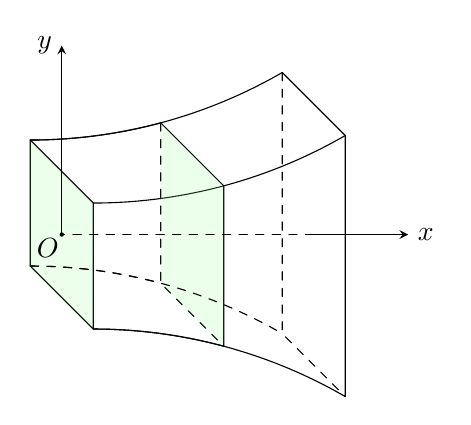
\begin{tikzpicture}[line join=round, line cap=round,>=stealth,scale=0.8,rotate=-90]
	\path 
	(0,0) coordinate (A)	
	(2,0) coordinate (B)
	(3,1) coordinate (C)
	(1,1) coordinate (D)
	(1.5,0.5) coordinate (F)
	(1.5,4.5) coordinate (G)		
	;
	\draw (A)--(B)--(C)--(D)--(A);
	\fill[color=green!40,opacity=0.2] (A)--(B)--(C)--(D);
			
	\draw[dashed] (B) arc (180:165:8) coordinate (B1);
	\draw (C) arc (180:165:8) coordinate (C1);
	\draw (A) arc (0:15:8) coordinate (A1);
	\draw (D) arc (0:15:8)coordinate (D1);
	\draw[dashed] (A1)--(B1)--(C1);\draw (C1)--(D1)--(A1);
	\fill[color=green!40,opacity=0.2] (A1)--(B1)--(C1)--(D1);
			
	\draw[dashed] (B) arc (180:150:8) coordinate (B2);
	\draw (C) arc (180:150:8) coordinate (C2);
	\draw (A) arc (0:30:8) coordinate (A2);
	\draw (D1) arc (15:30:8)coordinate (D2);
	\draw[dashed] (A2)--(B2)--(C2);\draw (C2)--(D2)--(A2);
	\draw [->] (1.5,4.5)--(1.5,6) node[right]{$x$};
	\draw [->] (1.5,0.5)--(-1.5,0.5) node[left]{$y$};
	\draw [dashed](G)--(F); 
	\fill (1.5,0.5) circle(1pt) node[shift=(-135:0.25)]{$O$};
	\end{tikzpicture}
	\end{center}
\begin{itemchoice}
	\itemch Vì chiều cao của thùng là $6$ dm nên $0\leq x\leq 6$.
	\itemch Từ giả thiết, ta có đường parabol $(P)$ có đỉnh là $I(0;1)$ nên có phương trình dạng $y=ax^2+1$.\\
	Mặt khác $(P)$ qua điểm $(6;2)$ nên $2=a\cdot 6^2+1 \Leftrightarrow a=\dfrac{1}{36}$.\\
	Vậy $(P)\colon y=\dfrac{1}{36}x^2+1$.
	\itemch Bề mặt nước ở độ cao $x$ dm là một hình vuông có cạnh bằng $2y=2\left(\dfrac{1}{36}x^2+1\right)=\dfrac{1}{18}x^2+2$.\\
	Vậy diện tích bề mặt nước tương ứng là $S=\left(\dfrac{1}{18}x^2+2\right)^2$.
	\itemch Dung tích của thùng là 
	\[V=\displaystyle \int\limits_{0}^{6}S(x)\mathrm{\,d}x=\displaystyle \int\limits_{0}^{6}\left(\dfrac{1}{18}x^2+2\right)^2\mathrm{\,d}x=\left(\dfrac{1}{1620}x^5+\dfrac{2}{27}x^3+4x\right)\bigg|_0^6=\dfrac{224}{5}= 44{,}8 (\text{dm}^3)= 44{,}8 (\text{lít}).\]
\end{itemchoice}
}
\end{ex}
\begin{ex}%[THPT 2025, Phát triển đề số 3]%[Nguyễn Cường]%[2D4V2-6]
	Một tàu ngầm nghiên cứu tự hành bắt đầu lặn xuống từ vị trí $A$ trên mặt biển để khảo sát một rảnh đại dương. Trong hệ trục $Oxyz$ (với mặt biển là mặt phẳng $(Oxy)$, trục $Oz$ là trục độ sâu, hướng thẳng đứng xuống dưới), vị trí $A$ có tọa độ $(50;100;0)$. Tàu di chuyển thẳng với vận tốc tại thời điểm $t$ (phút) được cho bởi công thức $v(t)=\alpha t+4$ (m/phút), với $\alpha$ là hằng số dương và $t\ge 0$. Hướng di chuyển của tàu có các đặc điểm sau:
	\begin{itemize}
		\item Vectơ đơn vị chỉ phương $\overrightarrow{u}=(0;b;c)\ne \overrightarrow{0}$.
		\item Hướng di chuyển vuông góc với vectơ $\overrightarrow{n}=(0;1;-2)$.
		\item Tàu đang lặn xuống.
	\end{itemize}
	Biết rằng tại thời điểm $t=10$\,phút, vận tốc của tàu đạt $9$\,m/phút.
	\choiceTF
	{\True $b=2c$}
	{\True Hằng số công thức vận tốc là $\alpha=0{,}5$}
	{\True Hướng di chuyển của tàu tạo với mặt biển một góc nhỏ hơn $30^\circ$}
	{Sau $20$ phút, tàu đến điểm $B$ có độ sâu lớn hơn $150$\,m}
	\loigiai{
		\begin{itemchoice}
			\itemch Ta có $\overrightarrow{u}\cdot\overrightarrow{n}=0\Leftrightarrow b-2c=0\Leftrightarrow b=2c$.
			\itemch Tại thời điểm $t=10$ thì $v(10)=9\Leftrightarrow 10\alpha+4=9\Leftrightarrow \alpha=0{,}5$.
			\itemch Do $\overrightarrow{u}$ là vectơ đơn vị nên $b^2+c^2=1\Rightarrow 5c^2=1\Leftrightarrow c=\dfrac{\sqrt{5}}{5}>0$ vì tàu lặn xuống.\\
			Suy ra vectơ $\overrightarrow{u}=\left(0;\dfrac{2\sqrt{5}}{5};\dfrac{\sqrt{5}}{5}\right)$.\\
			Gọi $\beta$ là góc tạo bởi phương di chuyển của tàu và mặt biển, ta có
			\[\sin\beta=\dfrac{\left|\overrightarrow{u}\cdot\overrightarrow{k}\right|}{\left|\overrightarrow{u}\right|\cdot\left|\overrightarrow{k}\right|}=\dfrac{\sqrt{5}}{5}.\]
			Suy ra $\beta\approx 26{,}57^\circ<30^\circ$.
			\itemch Quãng đường đi được sau $20$ phút của tàu là $\displaystyle\int\limits_0^{20}(0{,}5t+4)\mathrm{\,d}t=180$\,(m).\\
			Khi đó, ta có 
				$$\overrightarrow{AB}=180\overrightarrow{u}\Leftrightarrow\heva{&x_B-50=0\\&y_B-100=72\sqrt{5}\\&z_B-0=36\sqrt{5}}\Leftrightarrow\heva{&x_B=50\\&y_B=100+72\sqrt{5}\\&z_B=36\sqrt{5}.}$$
			Vậy độ sâu của $B$ là $z_B=36\sqrt{5}\approx 80{,}5<150$.
		\end{itemchoice}
	}
\end{ex}

\begin{ex}%[THPT 2025, Phát triển đề số 3]%[Nguyễn Cường]%[2D6H2-4]
	Một loại bệnh hiếm có tỉ lệ người mắc trong cộng đồng là $2\%$. Để chuẩn đoán bệnh này người ta sử dụng một phương pháp xét nghiệm. Phương pháp này có các đặc điểm sau
	\begin{itemize}
		\item Nếu một người mắc bệnh, xác suất để xét nghiệm cho kết quả dương tính là $98\%$.
		\item Nếu một người không mắc, xác suất để xét nghiệm cho kết quả dương tính (dương tính giả) là $5\%$.
	\end{itemize}
	Chọn ngẫu nhiên một người trong cộng đồng để thực hiện xét nghiệm.
	\choiceTF
	{\True Xác suất người được chọn không mắc bệnh là $0{,}98$}
	{\True Xác suất để người được chọn có kết quả xét nghiệm âm tính, biết rằng người đó không mắc bệnh là $0{,}95$}
	{\True Xác suất để người được chọn có kết quả dương tính là $0{,}0686$}
	{Xác suất để một người thực sự mắc bệnh, biết rằng kết quả xét nghiệm của người đó là dương tính, lớn hơn $30\%$}
	\loigiai{
		Gọi $A$ là biến cố \lq\lq người được chọn mắc bệnh\rq\rq;\\
		$B$ là biến cố \lq\lq người được chọn xét nghiệm dương tính\rq\rq.\\
		Theo giả thiết, ta có sơ đồ hình cây sau đây
		\begin{center}
			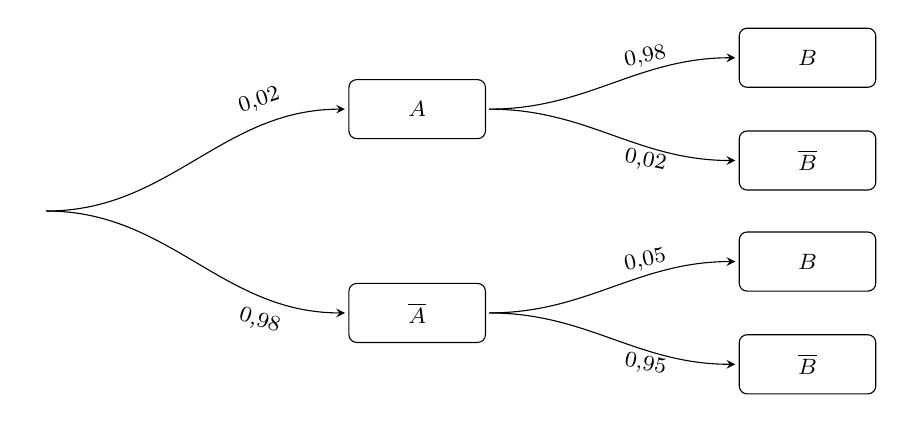
\begin{tikzpicture}[line join = round, line cap = round, >=stealth, font=\footnotesize, scale=1]
				\def\gocm{15}\def\gocn{7.5}\def\r{5}
				\tikzset{s/.style={outer sep=0.5 mm,draw=black,rectangle,minimum width=1.5cm,text width=1.5cm,align=center,rounded corners=1mm,minimum height=0.75cm}}
				
				\path(0,0)node(O){}++(\gocm:\r)node[s](A1){$A$}++(\gocn:\r)node[s](A2){$B$};
				\path(A1)++({-\gocn}:\r)node[s](a2){$\overline{B}$};
				\path(O)++(-\gocm:\r)node[s](B1){$\overline{A}$}++(\gocn:\r)node[s](B2){$B$};
				\path(B1)++({-\gocn}:\r)node[s](b2){$\overline{B}$};
				\foreach \x/\y in {O/A1,A1/A2,A1/a2,O/B1,B1/B2,B1/b2}{
					\draw[->,out=0,in=180] (\x.east)to(\y.west);	}
				\path
				(O)--(A1.west)node[pos=0.75,above=2mm,sloped]{$0{,}02$} (A1.east)--(A2.west)node[pos=0.65,above,sloped]{$0{,}98$}
				(A1.east)--(a2.west)node[pos=0.65,below,sloped]{$0{,}02$}
				(O)--(B1.west)node[pos=0.75,below=2mm,sloped]{$0{,}98$}
				(B1.east)--(B2.west)node[pos=0.65,above,sloped]{$0{,}05$}
				(B1.east)--(b2.west)node[pos=0.65,below,sloped]{$0{,}95$}
				;
			\end{tikzpicture}
		\end{center}
		\begin{itemchoice}
			\itemch  Xác suất người được chọn không mắc bệnh là $\mathrm{P}\left(\overline{A}\right)=1-\mathrm{P}(A)=1-0{,}02=0{,}98$.
			\itemch  Xác suất người được chọn có kết quả xét nghiệm âm tính, biết rằng người đó không mắc bệnh là $$\mathrm{P}\left(\overline{B}\mid\overline{A}\right)=1-\mathrm{P}\left(B|\overline{A}\right)=1-0{,}05=0{,}95.$$
			\itemch  Xác xuất để người được chọn có kết quả dương tính là
			\allowdisplaybreaks
			\begin{eqnarray*}
				\mathrm{P}(B)&=&\mathrm{P}(A)\cdot \mathrm{P}(B\mid A) + \mathrm{P}\left(\overline{A}\right)\cdot \mathrm{P}\left(\overline{B}\mid A\right)\\
				&=& 0{,}02 \cdot 0{,}98 + 0{,}98 \cdot 0{,}05 = 0{,}0686.
			\end{eqnarray*}
			\itemch  Xác suất để một người thực sự mắc bệnh, biết rằng kết quả xét nghiệm của người đó là dương tính
			$$\mathrm{P}(A\mid B)=\dfrac{\mathrm{P}(B\mid A)\cdot \mathrm{P}(A)}{\mathrm{P}(B)}=\dfrac{0{,}02 \cdot 0{,}98}{0{,}0686}=\dfrac{2}{7}.$$
			Vậy $\mathrm{P}(A\mid B)<0{,}3$.
		\end{itemchoice}
	}
\end{ex}
\Closesolutionfile{ans}
\indapan{2}{ans/2-TN-2025-PT3-DS}

% \caukq
\Opensolutionfile{ans}[ans/2-TN-2025-PT3-KQ]

\begin{ex}%[PT đề thi TN 2025]%[Xuân Tín Huỳnh]%[0D0C2-7]
	Bạn Nam tham gia cuộc thi giải một mật thư. Theo quy tắc của cuộc thi, người chơi cần chọn ra sáu số từ tập $S=\{2; 3; 4; 5; 6; 7; 8; 9;10\}$ và xếp mỗi số vào đúng một vị trí trong sáu vị trí $A$, $B$, $C$, $D$, $M$, $N$, $P$, $Q$ sao cho mỗi vị trí chỉ được xếp một số như hình bên dưới:
\begin{center}
\begin{tikzpicture}[scale=0.8, font=\footnotesize,line join=round, line cap=round, >=stealth] 
		\path
		(0,0) coordinate (O)
		(-4,2) coordinate (A)
		(4,-2) coordinate (C)
		(-4,-2) coordinate (D)
		(4,2) coordinate (B)
		(0,2) coordinate (M)
		(4,0) coordinate (N)
		(0,-2) coordinate (P)
		(-4,0) coordinate (Q)
		(-0.5,2) coordinate (M1)
		(0.5,2) coordinate (M2)
		(4,0.5) coordinate (N1)
		(4,-0.5) coordinate (N2)
		(0.5,-2) coordinate (P1)
				(-0.5,-2) coordinate (P2)
		(-4,-.5) coordinate (Q1)	
		(-4,.5) coordinate (Q2)			
		($(B)!0.5!(A)$) coordinate (T1)
		($(B)!0.5!(C)$) coordinate (T2)
		($(C)!0.5!(D)$) coordinate (T3)
		($(D)!0.5!(A)$) coordinate (T4)
		($(A)!0.5!(O)$) coordinate (T5)
		($(B)!0.5!(O)$) coordinate (T6)
		($(C)!0.5!(O)$) coordinate (T7)
		($(D)!0.5!(O)$) coordinate (T8)
		(-3.5,2) coordinate (A1)
		(-4,1.5) coordinate (A2)
		(-3.5,-2) coordinate (D1)
		(-4,-1.5) coordinate (D2)
		(4,-1.5) coordinate (C1)
		(3.5,-2) coordinate (C2)
		(3.5,2) coordinate (B1)
		(4,1.5) coordinate (B2)
		(3.552786405,1.776393202) coordinate (B3)	
		(-3.552786405,-1.776393202) coordinate (D3)	
		(3.552786405,-1.776393202) coordinate (C3)
		(-3.552786405,1.776393202) coordinate (A3)
		(0.4472135955,0.2236067978) coordinate (B4)
		(0.4472135955,-0.2236067978) coordinate (C4)
		(-0.4472135955,-0.2236067978) coordinate (D4)
		(-0.4472135955,0.2236067978) coordinate (A4);
		\foreach \x/\g in {O/0,A/180,B/-90,C/-90,D/0,M/0,N/0,P/0,Q/0}\draw[fill=white] (\x) node{$\x$};
		
		\draw (A1) -- (M1) (M2)--(B1) (B2)--(N1) (N2)--(C1)  (D2)--(Q1) (Q2)-- (A2)  (D1)--(P2) (P1)--(C2); 
		\draw (O) circle (.5);
		\draw (A) circle (.5);
		\draw (B) circle (.5);
		\draw (C) circle (.5);
		\draw (D) circle (.5);
		\draw (M) circle (.5);
		\draw (N) circle (.5);
		\draw (P) circle (.5);
		\draw (Q) circle (.5);		
	\end{tikzpicture}
\end{center}
 Mật thư sẽ được giải nếu các bộ ba số xuất hiện ở những bộ ba vị trí $(A, M, B)$; $(B, N, C)$; $(C, P, D)$; $(D, Q, A)$; $(A, O, C)$; $(B, O, D)$ tạo thành các cấp số cộng theo thứ tự đó. Bạn Nam chọn ngẫu nhiên $8$ số trong tập $S$ và xếp ngẫu nhiên vào các vị trí được yêu cầu. Gọi xác suất để bạn Nam giải được mật thư ở lần chọn và xếp đó là $a$. Giá trị của $\dfrac{1}{100a}$ bằng bao nhiêu (làm tròn đến hàng đơn vị)?
	\shortans{907}
\loigiai{
	Số cách chọn ra $8$ số và xếp ngẫu nhiên là $\mathrm{C}_9^8 \cdot 8!=\mathrm{A}_9^8$.\\
	Vì các bộ ba số xuất hiện ở những bộ ba vị trí $(A, M, B)$; $(B, N, C)$; $(C, P, D)$; $(D, Q, A)$ ; $(A, O, C)$; $(B, O, D)$ tạo thành các cấp số cộng theo thứ tự đó nên $\heva{&A+B=2 M;\\ &B+C=2 N;\\ &C+A=2 O\\&C+D=2P\\&D+B=2O\\&D+A=2Q} \Rightarrow$ mỗi cặp $(A ; B)$, $(B ; C)$, $(C ; A)$; $(B ; D)$, $(C ; D)$; $(D;A)$ cùng tính chẵn lẻ hay $A$, $B$, $C$; $D$ cùng tính chẵn lẻ.
	\begin{enumerate}[TH 1.]
\item Bộ $(A;B;C;D)$ cùng lẻ. Khi đó $(A;B;C;D)$ là $(3;5;7;9)$.
		\begin{enumerate}[TH i.]
			\item 	Bộ $(A;B;C;D)$ dạng $(3;5;7;9)$ không xảy ra vì có $\dfrac{3+9}{2}=\dfrac{5+7}{2}$
			\item Bộ $(A;B;C;D)$ dạng $(3;7;5;9)$ cũng không xảy ra vì số có $\dfrac{3+7}{2}=5$.
			\item Tương tự các bộ $(3;5;9;7)$ cũng loại vì có $\dfrac{5+9}{2}=7$.
		\end{enumerate}
\item 	Bộ $(A;B;C;D)$ cùng chẵn.
		\begin{enumerate}[TH i.]
		\item 	Bộ $(A;B;C;D)$ dạng $(2;4;6;8)$ không xảy ra vì số $(2;4;6;8)$ có $\dfrac{4+5}{2}=\dfrac{2+8}{2}$;  $(2;6;4;8)$ có $\break \dfrac{2+8}{2}=\dfrac{4+6}{2}$;  $(2;4;8;6)$ có $\dfrac{2+6}{2}=4$; và các hoán vị khác của bộ $(2;4;6;8)$ đều loại.
		\item Bộ $(A;B;C;D)$ dạng $(2;4;6;10)$ cũng không xảy ra vì số $(2;4;6;10)$ có $\dfrac{2+10}{2}=6$;  $(2;6;10;4)$ có $\dfrac{2+6}{2}=4$;  $(2;6;4;10)$ có $\dfrac{2+6}{2}=4$; và các hoán vị khác của bộ $(2;4;6;10)$ đều loại.
 		\item Tương tự các bộ $(2;6;8;10)$, $(4;6;8;10)$ cũng loại.
 		\item Bộ $(A;B;C;D)$ dạng $(2;4;8;10)$. Ta thử các trường hợp chỉ có bộ thứ tự $(2;8;10;4)$, $(4;2;8;10)$, $(10;4;2;8)$, $(8;10;4;2)$ là thỏa mãn.\\
 		Với mỗi bộ $(A;B;C;D)$ được chọn thì sẽ có duy nhất cách chọn các số cho ô $M$, $N$, $P$, $Q$.
	\end{enumerate}
	\end{enumerate}
	Vậy có tất cả $4$ cách chọn và sắp xếp thỏa mãn.\\
		Khi đó $a=\dfrac{4}{\mathrm{A}_9^8}=\dfrac{1}{90\,720} \Rightarrow \dfrac{1}{100a}\approx 907$.
}
\end{ex}

\begin{ex}%[2D1V3-6]%[PT đề thi TN 2025]%[Xuân Tín Huỳnh]
	Nhà máy $A$ chuyên sản xuất một loại sản phẩm cung cấp cho nhà máy $B$. Hai nhà máy thoả thuận rằng, hàng tháng nhà máy $A$ cung cấp cho nhà máy $B$ số lượng sản phẩm theo đơn đặt hàng của $B$ (tối đa $100$ tấn sản phẩm). Nếu số lượng đặt hàng là $x$ tấn sản phẩm thì giá bán cho mỗi tấn sản phẩm là $P(x)=45-0{,}001 x^2$ (triệu đồng). Chi phí để $A$ sản xuất $x$ tấn sản phẩm trong một tháng gồm $100$ triệu đồng chi phí cố định và $30$ triệu đồng cho mỗi tấn sản phẩm. Nhà máy $A$ cần bán cho nhà máy $B$ bao nhiêu tấn sản phẩm mỗi tháng để lợi nhuận thu được lớn nhất? (làm tròn kết quả đến hàng phần mười).
	\shortans{70,7}
	\loigiai{
		Số tiền (triệu đồng) mà nhà máy $A$ thu được từ việc bán $x$ tấn sản phẩm $(0 \leq x \leq 100)$ cho nhà máy $B$ là 
		$$
		R(x)=x \cdot P(x)=x\left(45-0{,}001 x^2\right)=45 x-0{,}001 x^3.
		$$
		Chi phí (triệu đồng) để $A$ sản xuất $x$ tấn sản phẩm trong một tháng là
		$$
		C(x)=100+30 x.
		$$
		Lợi nhuận (triệu đồng) mà nhà máy $A$ thu được là
		$$
		P(x)=R(x)-C(x)=x\left(45-0{,}001 x^2\right)-(100+30 x)=-0{,}001 x^3+15 x-100.
		$$
		Xét hàm số 
		$$
		P(x)=-0{,}001 x^3+15 x-100 \quad\text{với } (0 \leq x \leq 100).
		$$
		Ta có
		$$
		P'(x)=-0{,}003 x^2+15=0 
		\Leftrightarrow x^2=5000 
		\Leftrightarrow x=50 \sqrt{2}.
		$$
		Mặt khác
		$$
		P(0)=-100;\quad
		P\left(50 \sqrt{2}\right)=500 \sqrt{2}-100 \approx 607;\quad
		P(100)=400.
		$$
		Vậy nhà máy $A$ thu được lợi nhuận lớn nhất là $607$ triệu đồng khi bán $50 \sqrt{2} \approx 70{,}7$ tấn sản phẩm cho nhà máy $B$ mỗi tháng.
	}
\end{ex}

\begin{ex}%[0D2V2-3]%[PT đề thi TN 2025]%[Xuân Tín Huỳnh]
	Người ta dự định dùng hai loại nguyên liệu để chiết xuất ít nhất $280$ kg chất $A$ và $18$ kg chất $B$. Với một tấn nguyên liệu loại $I$, người ta có thể chiết xuất được $40$ kg chất $A$ và $1{,}2$ kg chất $B$. Với một tấn nguyên liệu loại $II$, người ta có thể chiết xuất được $20$ kg chất $A$ và $3$ kg chất $B$. Giá mỗi tấn nguyên liệu loại $I$ là $4$ triệu đồng và loại $II$ là $3$ triệu đồng. Hỏi người ta phải dùng bao nhiêu tấn nguyên liệu loại $I$ để chi phí mua nguyên liệu là ít nhất mà vẫn đạt được mục tiêu đề ra? Biết rằng cơ sở cung cấp nguyên liệu chỉ có thể cung cấp tối đa $10$ tấn nguyên liệu loại $I$ và $9$ tấn nguyên liệu loại $II$.
	\shortans{5}
	\loigiai{
		Gọi $x$ và $y$ lần lượt là số tấn nguyên liệu loại $I$ và loại $II$ mà người ta cần dùng. Khi đó khối lượng chất $A$ chiết xuất được là $40x+20y$ (kg). Khối lượng chất $B$ chiết xuất được là $1{,}2x+3y$ (kg).\\
		Từ giả thiết ta có hệ bất phương trình $\begin{cases}
			40x+20y \ge 280\\
			1{,}2x+3y \ge 18\\
			0\le x \le 10\\
			0\le y \le 9
		\end{cases} \Leftrightarrow \begin{cases}
			2x+y \ge 14\\
			1{,}2x+3y \ge 18\\
			0\le x \le 10\\
			0\le y \le 9.
		\end{cases}$\\
		Hơn nữa, số tiền người ta phải trả để mua nguyên liệu là $F(x; y)=4x+3y$ (triệu đồng). Vậy bài toán trở thành tìm giá trị nhỏ nhất của $F(x;y)$ với $(x; y)$ thoả mãn hệ bất phương trình bậc nhất hai ẩn ở trên.
		\immini
		{\begin{itemize}
				\item Xác định miền nghiệm của hệ bất phương trình bậc nhất hai ẩn trên. Miền nghiệm là miền tứ giác $ABCD$ (kể cả biên) với $A(5;4)$, $B(10;2)$, $C(10;9)$, $D(2,5;9)$.
				\item Tính giá trị của $F$ tại các đỉnh của tứ giác $ABCD$.\\
				Ta có $F(5;4)=32$, $F(10;2)=46$, $F(10;9)=67$, $F(2{,}5;9)=37$.
		\end{itemize}}
		{\begin{tikzpicture}[>=stealth,line join=round,line cap=round,font=\footnotesize,scale=0.6]
				\draw[->] (-0.5,0)--(10.5,0)node[below right]{$x$};
				\draw[->] (0,-0.5)--(0,9.5) node[left]{$y$};
				\path[pattern=grid] (2.25,9.5)-|(-0.5,-0.5)--(7.25,-0.5)--cycle;
				\draw (2.25,9.5)--(7.25,-0.5);
				\path[pattern=horizontal lines] (-0.5,6.2)|-(10.5,-0.5)--(10.5,1.8)--cycle;
				\draw (-0.5,6.2)--(10.5,1.8);
				\path[pattern=horizontal lines] (10.5,9.5)rectangle(10,-0.5);
				\draw (10,-0.5)--(10,9.5);
				\path[pattern=crosshatch] (-0.5,9.5)rectangle(10.5,9);
				\draw (-0.5,9)--(10.5,9);
				\path (0,0)coordinate[label=below left:$O$](O) (5,4)coordinate[label=above right:$A$](A) (10,2)coordinate[label=above left:$B$](B) (10,9)coordinate[label=below left:$C$](C) (2.5,9)coordinate[label=below right:$D$](D);
				\foreach \diem in {O,A,B,C,D} \fill[black](\diem)circle(1.5pt);		
		\end{tikzpicture}}
		\vspace*{0.3cm}
		\noindent
		So sánh các giá trị này ta thấy $F(5;4)$ là nhỏ nhất. Do đó, giá trị nhỏ nhất của $F(x;y)$ với $(x;y)$ thoả mãn hệ bất phương trình trên là $F(5;4)=32$.\\		
		Vậy người ta cần mua $5$ tấn nguyên liệu loại $I$ và $4$ tấn nguyên liệu loại $II$ để chi phí là nhỏ nhất.
	}
\end{ex}
\begin{ex}%[Dự án Tex hoá đề Tốt nghiệp 2025 + Phát triển 05 đề]%[Viết Tường]%[1H8V6-6]
	Cho hình chóp $S.ABCD$ có đáy $ABCD$ là hình thoi với $\widehat{ABC}=60^{\circ}$ và $AB=5$. Biết rằng hình chiếu vuông góc của $S$ lên mặt phẳng $(ABCD)$ là trọng tâm $H$ của $\triangle ABC$ và $SH=\sqrt{3}$. Khoảng cách giữa hai đường thẳng $AC$ và $SD$ bằng bao nhiêu (không làm tròn kết quả của các phép tính trung gian, chỉ làm tròn kết quả cuối cùng đến hàng phần trăm)?
	\shortans{1,24}
	\loigiai
	{
		\immini
	{
		Gọi $O=AC \cap BD$, kẻ $OF\perp SD$ với $(F \in SD)$ và kẻ $HE \parallel OF$ với $(E \in SD)$.\\
		Ta có $\heva{&AC\perp BD\\&AC\perp SH}\Rightarrow AC\perp (SBD)$.\\
		Suy ra $AC\perp OF$ do đó $\mathrm{d}(AC,SD)=OF$.\\
		Ta có $\dfrac{OF}{HE}=\dfrac{DO}{DH}=\dfrac{3}{4} \Rightarrow OF=\dfrac{3}{4} HE$.\\ Tam giác $ABC$ đều cạnh $5\Rightarrow HB=\dfrac{5}{\sqrt{3}} \Rightarrow HD=2HB=\dfrac{10}{\sqrt{3}}$.\\
		Vậy $OF=\dfrac{3}{4} HE=\dfrac{3}{4}\cdot\dfrac{SH\cdot HD}{\sqrt{SH^2+HD^2}}=\dfrac{3}{4}\cdot\dfrac{\sqrt{3}\cdot\tfrac{10}{\sqrt{3}}}{\sqrt{3+\tfrac{100}{3}}} \approx 1{,}24$.
	}
	{
		\begin{tikzpicture}[>=stealth,line join=round,line cap=round,font=\footnotesize,scale=0.75]
			\coordinate (A) at (0,0);
			\coordinate (B) at (-2,-2);
			\coordinate (D) at (5,0);
			\coordinate (C) at ($(B)+(D)-(A)$);
			\coordinate (O) at ($(A)!0.5!(C)$);
			\coordinate (M) at ($(B)!.5!(C)$);
			\coordinate (N) at ($(A)!.5!(B)$);
			\coordinate (H) at ($(A)!2/3!(M)$);
			\coordinate (S) at ($(H)+(0,5)$);
			\coordinate (E) at ($(S)!.45!(D)$);
			\coordinate (F) at ($(S)!.6!(D)$);
			\draw (S)--(B)--(C)--(D)--(S)--(C);
			\draw[dashed] (B)--(A)--(D) (A)--(S)--(H)--(E) (B)--(D) (A)--(C)--(N) (O)--(F) ;
			\foreach \d/\g in {A/180,B/190,C/-50,D/0,S/90,H/-90,E/70,O/-90,F/70}
			\fill[black](\d) circle (1pt)+(\g:.3)node{$\d$};
			\foreach\x/\y/\z in{S/H/D, D/E/H, D/F/O}\pic[draw,angle radius=6]{right angle=\x--\y--\z};
		\end{tikzpicture}
	}
	}
\end{ex}

\begin{ex}%[Dự án Tex hoá đề Tốt nghiệp 2025 + Phát triển 05 đề]%[Viết Tường]%[0D8V2-7]
	Có $5$ ngăn (trong một giá để sách) được đánh số thứ tự $1,2,3,4,5$ và chín quyển sách khác nhau. Bạn Bình xếp hết chín quyển sách vào $5$ ngăn sao cho mỗi ngăn có ít nhất một quyển sách và các quyển sách trong mỗi ngăn được xếp thẳng đứng thành một hàng ngang (gáy sách quay ra ngoài). Khi đã xếp xong chín quyển sách, hai cách xếp của bạn Bình được gọi là giống nhau nếu chúng thoả mãn đồng thời hai điều kiện sau đây:
	\begin{itemize}
		\item Số lượng sách trong từng ngăn giống nhau ở cả hai cách xếp.
		\item Thứ tự sách từ trái sang phải trong từng ngăn giống nhau ở cả hai cách xếp.
	\end{itemize}
	Gọi $T$ là số cách xếp đôi một khác nhau của bạn Bình. Tính giá trị của $\dfrac{T}{20\,736}$.
	\shortans{1225}
	\loigiai
	{
		Giữa $9$ quyển sách có $8$ chỗ trống. Số cách chia $9$ quyển sách vào $5$ ngăn sao cho mỗi ngăn có ít nhất một quyển sách bằng số cách đặt $4$ vách ngăn vào $8$ chỗ trống và bằng $\mathrm{C}_8^4=70$ cách.\\
		Ứng với mỗi cách chia sách thành các ngăn ta có $9!=362\,880$ cách xếp $9$ quyển sách.\\
		Vậy $T=362\,880\cdot 70\Rightarrow \dfrac{T}{20\,736}=1225$.
	}
\end{ex}

\begin{ex}%[12-MH-2-MH2025]%[MH-2025, Chu Hà]%[2D4V3-5]
Nghệ thuật làm gốm có lịch sử phát triển lâu đời và vẫn còn tồn tại cho đến ngày nay. Giả sử một bình gốm có mặt trong của bình là một mặt tròn xoay sinh ra khi cho phần đồ thị của hàm số $y=\dfrac{1}{175} x^2+\dfrac{3}{35} x+5$ $\left(0 \leq x \leq 30\right)$ ($x$, $y$ tính theo cm) quay tròn quanh bệ gốm có trục trùng với trục hoành $O x$. Hỏi để hoàn thành bình gốm đó ta cần sử dụng bao nhiêu cm$^3$ đất sét, biết rằng bình gốm đó có độ dày không đổi là $1$ cm.
\shortans[]{$94{,}2$}
\loigiai{
Thể tích phần bên trong của bình gốm là
\[V_1=\pi \displaystyle \int\limits_0^{30} \left(\dfrac{1}{175} x^2+\dfrac{3}{35} x+5\right)^2  \mathrm{\,d}x=240\pi \, (\text{cm}^3).\]
Thể tích của bình gốm bao gồm cả độ dày là
\[V_2=\pi \displaystyle \int\limits_0^{30} \left(\dfrac{1}{175} x^2+\dfrac{3}{35} x+5+1\right)^2  \mathrm{\,d}x=270\pi \, (\text{cm}^3).\]
Thể tích cần dùng để hoàn thành bình gốm là
\[V=V_2-V_1=270 \pi-240\pi=30 \pi =94{,}2 \, (\text{cm}^3).\]
}
\end{ex}
\Closesolutionfile{ans}
% \indapan{6}{ans/2-TN-2025-PT3-KQ}
